% !Mode:: "TeX:UTF-8" 



\BiSection{2.19}{Figures}

\fancyhead[R]{本题2.19由QC.Z完成}



解:

$V_{TH}=\Phi_{MS}+2\Phi_F+\frac{Q_{dep}}{C_{ox}}$\textcolor{blue}{(见半导体物理Neamen第四版P277的10.31c,$|Q_{SD}'(max)|$在276的10.27,$x_{dT}$在271的10.8)}

上式中$\Phi_{MS}$和$\Phi_F$是常量,所以阈值电压的任何改变都来自$\frac{Q_{dep}}{C_{ox}}$项,所以$\Delta V_{TH}=\Delta \frac{Q_{dep}}{C_{ox}}$

而

\begin{figure}[H] %H为当前位置,!htb为忽略美学标准,htbp为浮动图形
	\begin{minipage}{\linewidth}
		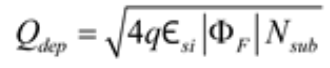
\includegraphics{2.19-1}
	\end{minipage}
\end{figure}



$V_{TH}=V_{TH0}+\gamma(\sqrt{|2\Phi_F+V_{SB}|}-\sqrt{|2\Phi_F|})$\textcolor{blue}{(见教材P20-2.23)}

其中$V_{TH0}=\Phi_{MS}+2\Phi_F+\frac{Q_{dep}}{C_{ox}}$


\begin{figure}[H] %H为当前位置,!htb为忽略美学标准,htbp为浮动图形
	\begin{minipage}{\linewidth}
		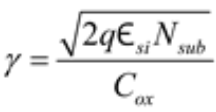
\includegraphics{2.19-2}
	\end{minipage}
\end{figure}







